\documentclass[11pt]{article}
\usepackage[utf8]{inputenc}
\usepackage{amsmath}
\usepackage{graphicx}
\usepackage{listings}
\usepackage{verbatim}
\usepackage{float}
\usepackage{xcolor}
\usepackage{subcaption}
\usepackage[english]{babel}
\usepackage{caption}
\usepackage{hyperref}
\usepackage{biblatex}
%\addbibresource{project2.bib}
\usepackage{setspace}
\usepackage{wrapfig}
\usepackage{lipsum}
\usepackage{amssymb}
\linespread{1.15}
\usepackage[a4paper, total={6.5in, 9in}]{geometry}


\hypersetup{
    colorlinks,
    linkcolor={red!50!black},
    citecolor={blue!50!black},
    urlcolor={blue!80!black}
}
\definecolor{codegreen}{rgb}{0,0.6,0}
\definecolor{codegray}{rgb}{0.5,0.5,0.5}
\definecolor{codepurple}{rgb}{0.58,0,0.82}
\definecolor{backcolour}{rgb}{0.95,0.95,0.92}
\definecolor{dkgreen}{rgb}{0,0.6,0}
\definecolor{gray}{rgb}{0.5,0.5,0.5}
\definecolor{mauve}{rgb}{0.58,0,0.82}

\lstdefinestyle{mystyle}{
    backgroundcolor=\color{backcolour},
    commentstyle=\color{codegreen},
    keywordstyle=\color{magenta},
    numberstyle=\tiny\color{codegray},
    stringstyle=\color{codepurple},
    basicstyle=\ttfamily\footnotesize,
    breakatwhitespace=false,
    breaklines=true,
    captionpos=b,
    keepspaces=true,
    numbers=left,
    numbersep=5pt,
    showspaces=false,
    showstringspaces=false,
    showtabs=false,
    tabsize=2
}

\lstset{style=mystyle}
\title{Project 3\\ }
\author{Filip Severin von der Lippe}
\date{\today}
\begin{document}
\maketitle
GitHub repository containing code and further instructions on how to reproduce the results of this report: \url{https://github.com/Fslippe/FYS-STK4155/tree/main/project3}
\url{https://openarchive.usn.no/usn-xmlui/handle/11250/2581934}
\url{https://www.kaggle.com/datasets/jsphyg/weather-dataset-rattle-package}
\begin{abstract}
\end{abstract}
\newpage
\tableofcontents
\newpage
\section{Introduction}
\section{Method}
\subsection{Structure of dataset} % (fold)
\label{sub:Structure of dataset}

The dataset found at \url{https://www.kaggle.com/datasets/jsphyg/weather-dataset-rattle-package} includes about 10 years of weather observations from numerous Australian weather stations. The observations include features such as temperature, wind, rainfall, and sunshine hours. A full overview of the dataset and its features can be found in table \ref{tab:features} in appendix \ref{app:dataset}. The main purpose of the dataset is to make a prediction based on today's weather if it is going to rain or not tomorrow. This prediction is either Yes or No, and we are therefore looking at a classification problem.



\subsection{Initializing of dataset}
The initializing and importing of the datasets require a few steps before we can train our models. These include importing the dataset to a pandas dataframe and removing all rows (days) which has at least one measurement missing. This allows for an easy way to load a training set to our models by excluding Not a Number (NaN) values and their possible negative influence on our models. This leaves us with less data to work with, but still a large amount.

The dataset comes with wind directions given in a 16-wind compass rose as seen in figure \ref{fig:compass}. This may cause some problems for some neural networks or other methods not built to handle letters or words as input. To solve this problem we translate them to labels from 0 to 15 going clockwise from North (0) to North North-West (15) as seen in table \ref{tab:compass}. The location of the weather station is given in names which also may cause problems for some models. This is solved by restricting each train and test sample to either a specific weather station or specific indexes corresponding to certain locations.
\begin{figure}[H]
    \centering
    
\includegraphics[width=.3\textwidth]{../figures/Brosen_windrose.png}
    \caption{16-wind compass rose used to describe wind directions. Labels are defined as N (North), S (South), W (West) and E (East).}
    \label{fig:compass}
\end{figure}
\begin{table}[H]
    \begin{small}
        \caption{Translation and labeling of the different wind directions into integers from 0 to 15.}
        \label{tab:compass}
        \begin{center}
            \begin{tabular}{|c|c|c|c|c|c|c|c|c|c|c|c|c|c|c|c|}
                \hline
                N & NNE & NE & ENE & E & ESE & SE & SSE & S & SSW & SW & WSW & W  & WNW & NW & NNW \\
                \hline
                0 & 1   & 2  & 3   & 4 & 5   & 6  & 7   & 8 & 9   & 10 & 11  & 12 & 13  & 14 & 15  \\
                \hline
            \end{tabular}
        \end{center}
    \end{small}
\end{table}


\subsection{Choosing data to analyze} % (fold)
\label{sub:Weather stations}
For our testing of the models and the dataset we start by looking at one single weather station Cobar. The data from this weather station containts 534 days which makes it one of the smaller datasets, enabling fast testing of our model. For further analysis we mainly look into three different weather stations. The choices are based on geographic position in hopes of finding a trained model's location dependency as well as its flexibility. We again look at the station Cobar, the station Coffs Harbour slightly to the east, and the north most weather station Darwin. These locations are highlighted below in figure \ref{fig:earth}. We also look into the dataset as a whole combining all the weather stations marked in figure \ref{fig:earth}
\begin{figure}[H]
    \centering
    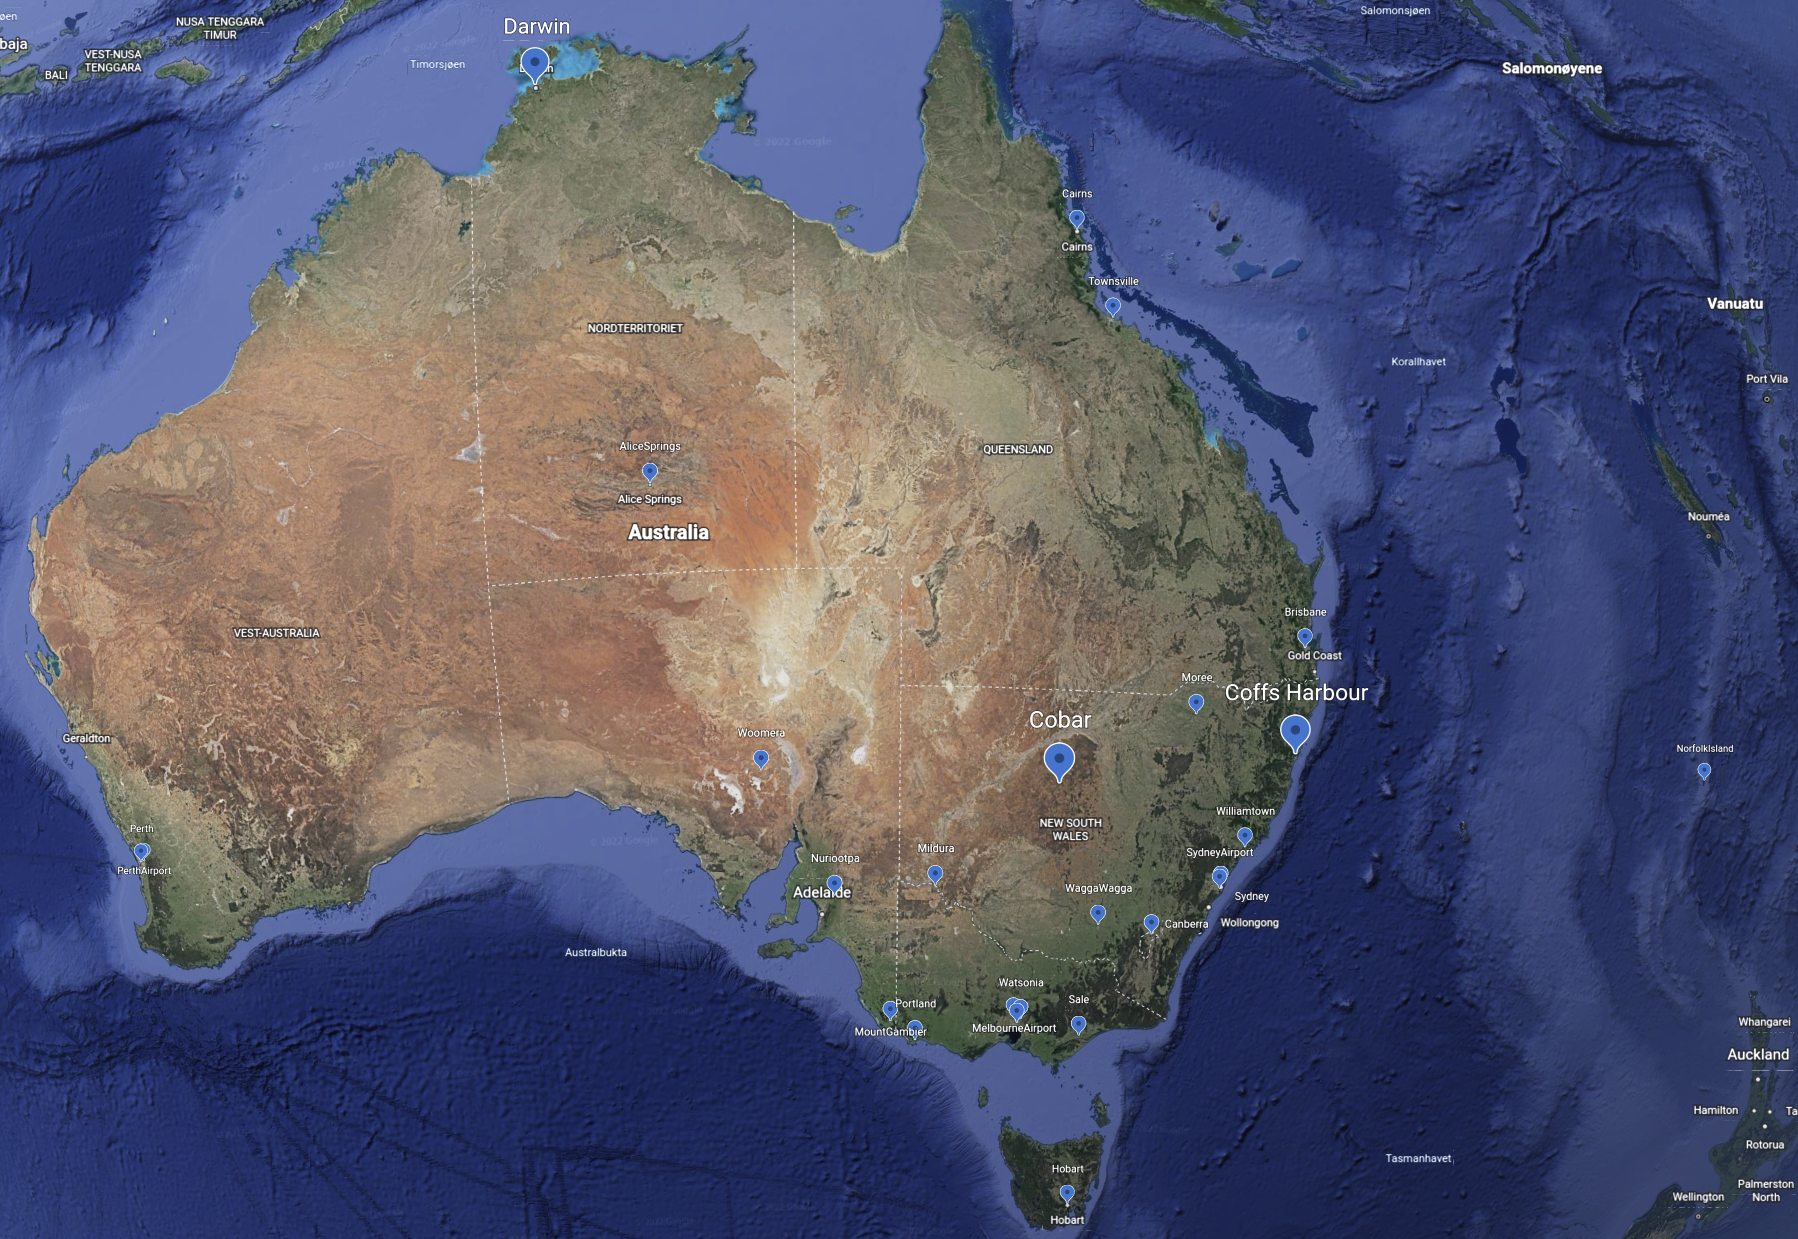
\includegraphics[width=\textwidth]{../figures/earth.png}
    \caption{Satellite image of Australia with all weather stations marked with blue points. The three stations Cobar, Darwin and Coffs Harbour which we will focus on are marked with larger points. \textit{Picture source: Screenshot from Google Earth dated 12. Dec. 2022.}}
    \label{fig:earth}
\end{figure}
% subsubsection Weather stations (end)




\section{Results}
To get a better understanding of the dataset we plot the correlation matrix as seen in figure \ref{fig:corr}
\begin{figure}[H]
    \centering
    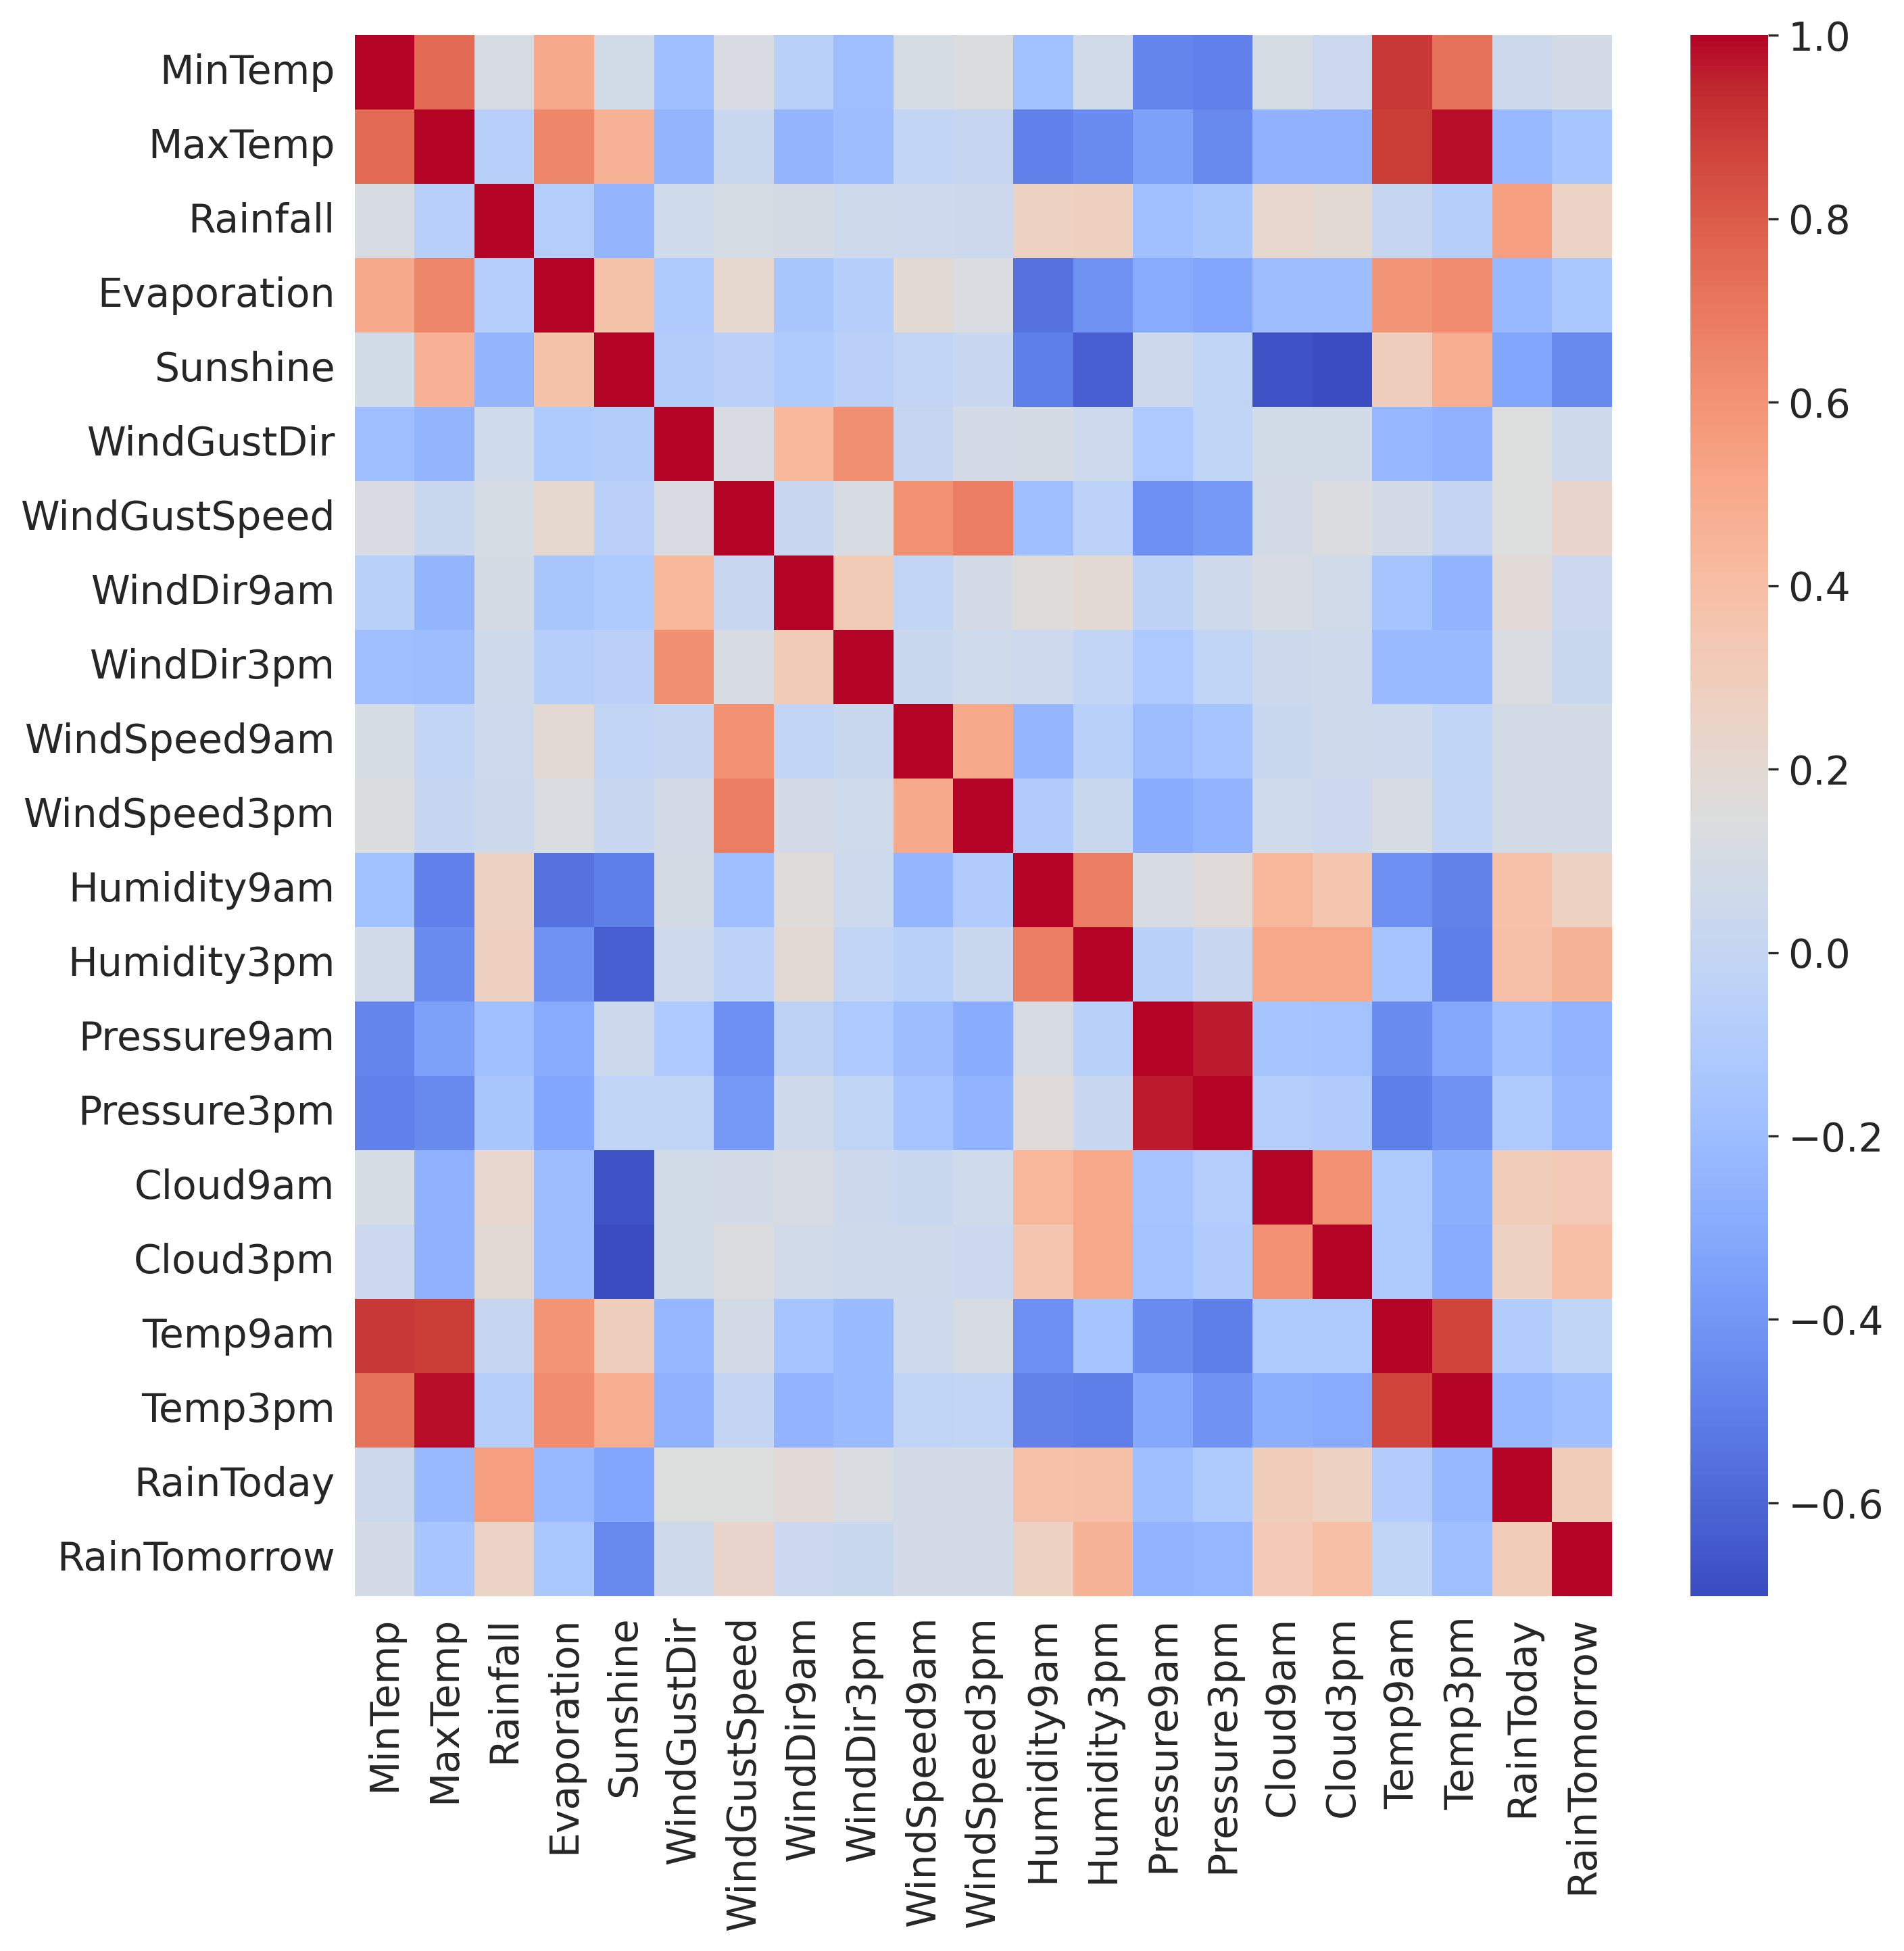
\includegraphics[width=0.8\textwidth]{../figures/correlation_heatmap_full.png}
    \caption{Correlation between the different features of the dataset.}
    \label{fig:corr}
\end{figure}

In our case of mainly looking at how today's weather influences tomorrow's weather is the bottom row or the rightmost column in figure \ref{fig:corr} what interests us. We see that the different features influences the feature "RainTomorrow" to different degrees. Number of sunshine hours is the feature with the most negative correlation while the humidity at 3pm is the feature with the most positive correlation.

In figure \ref{fig:features} we see how different weather stations deviate from the mean. We see sunshine hours in \ref{fig:sunshine} and humidity in \ref{fig:humidity}
\begin{figure}
    \begin{subfigure}{\textwidth}
        \centering
        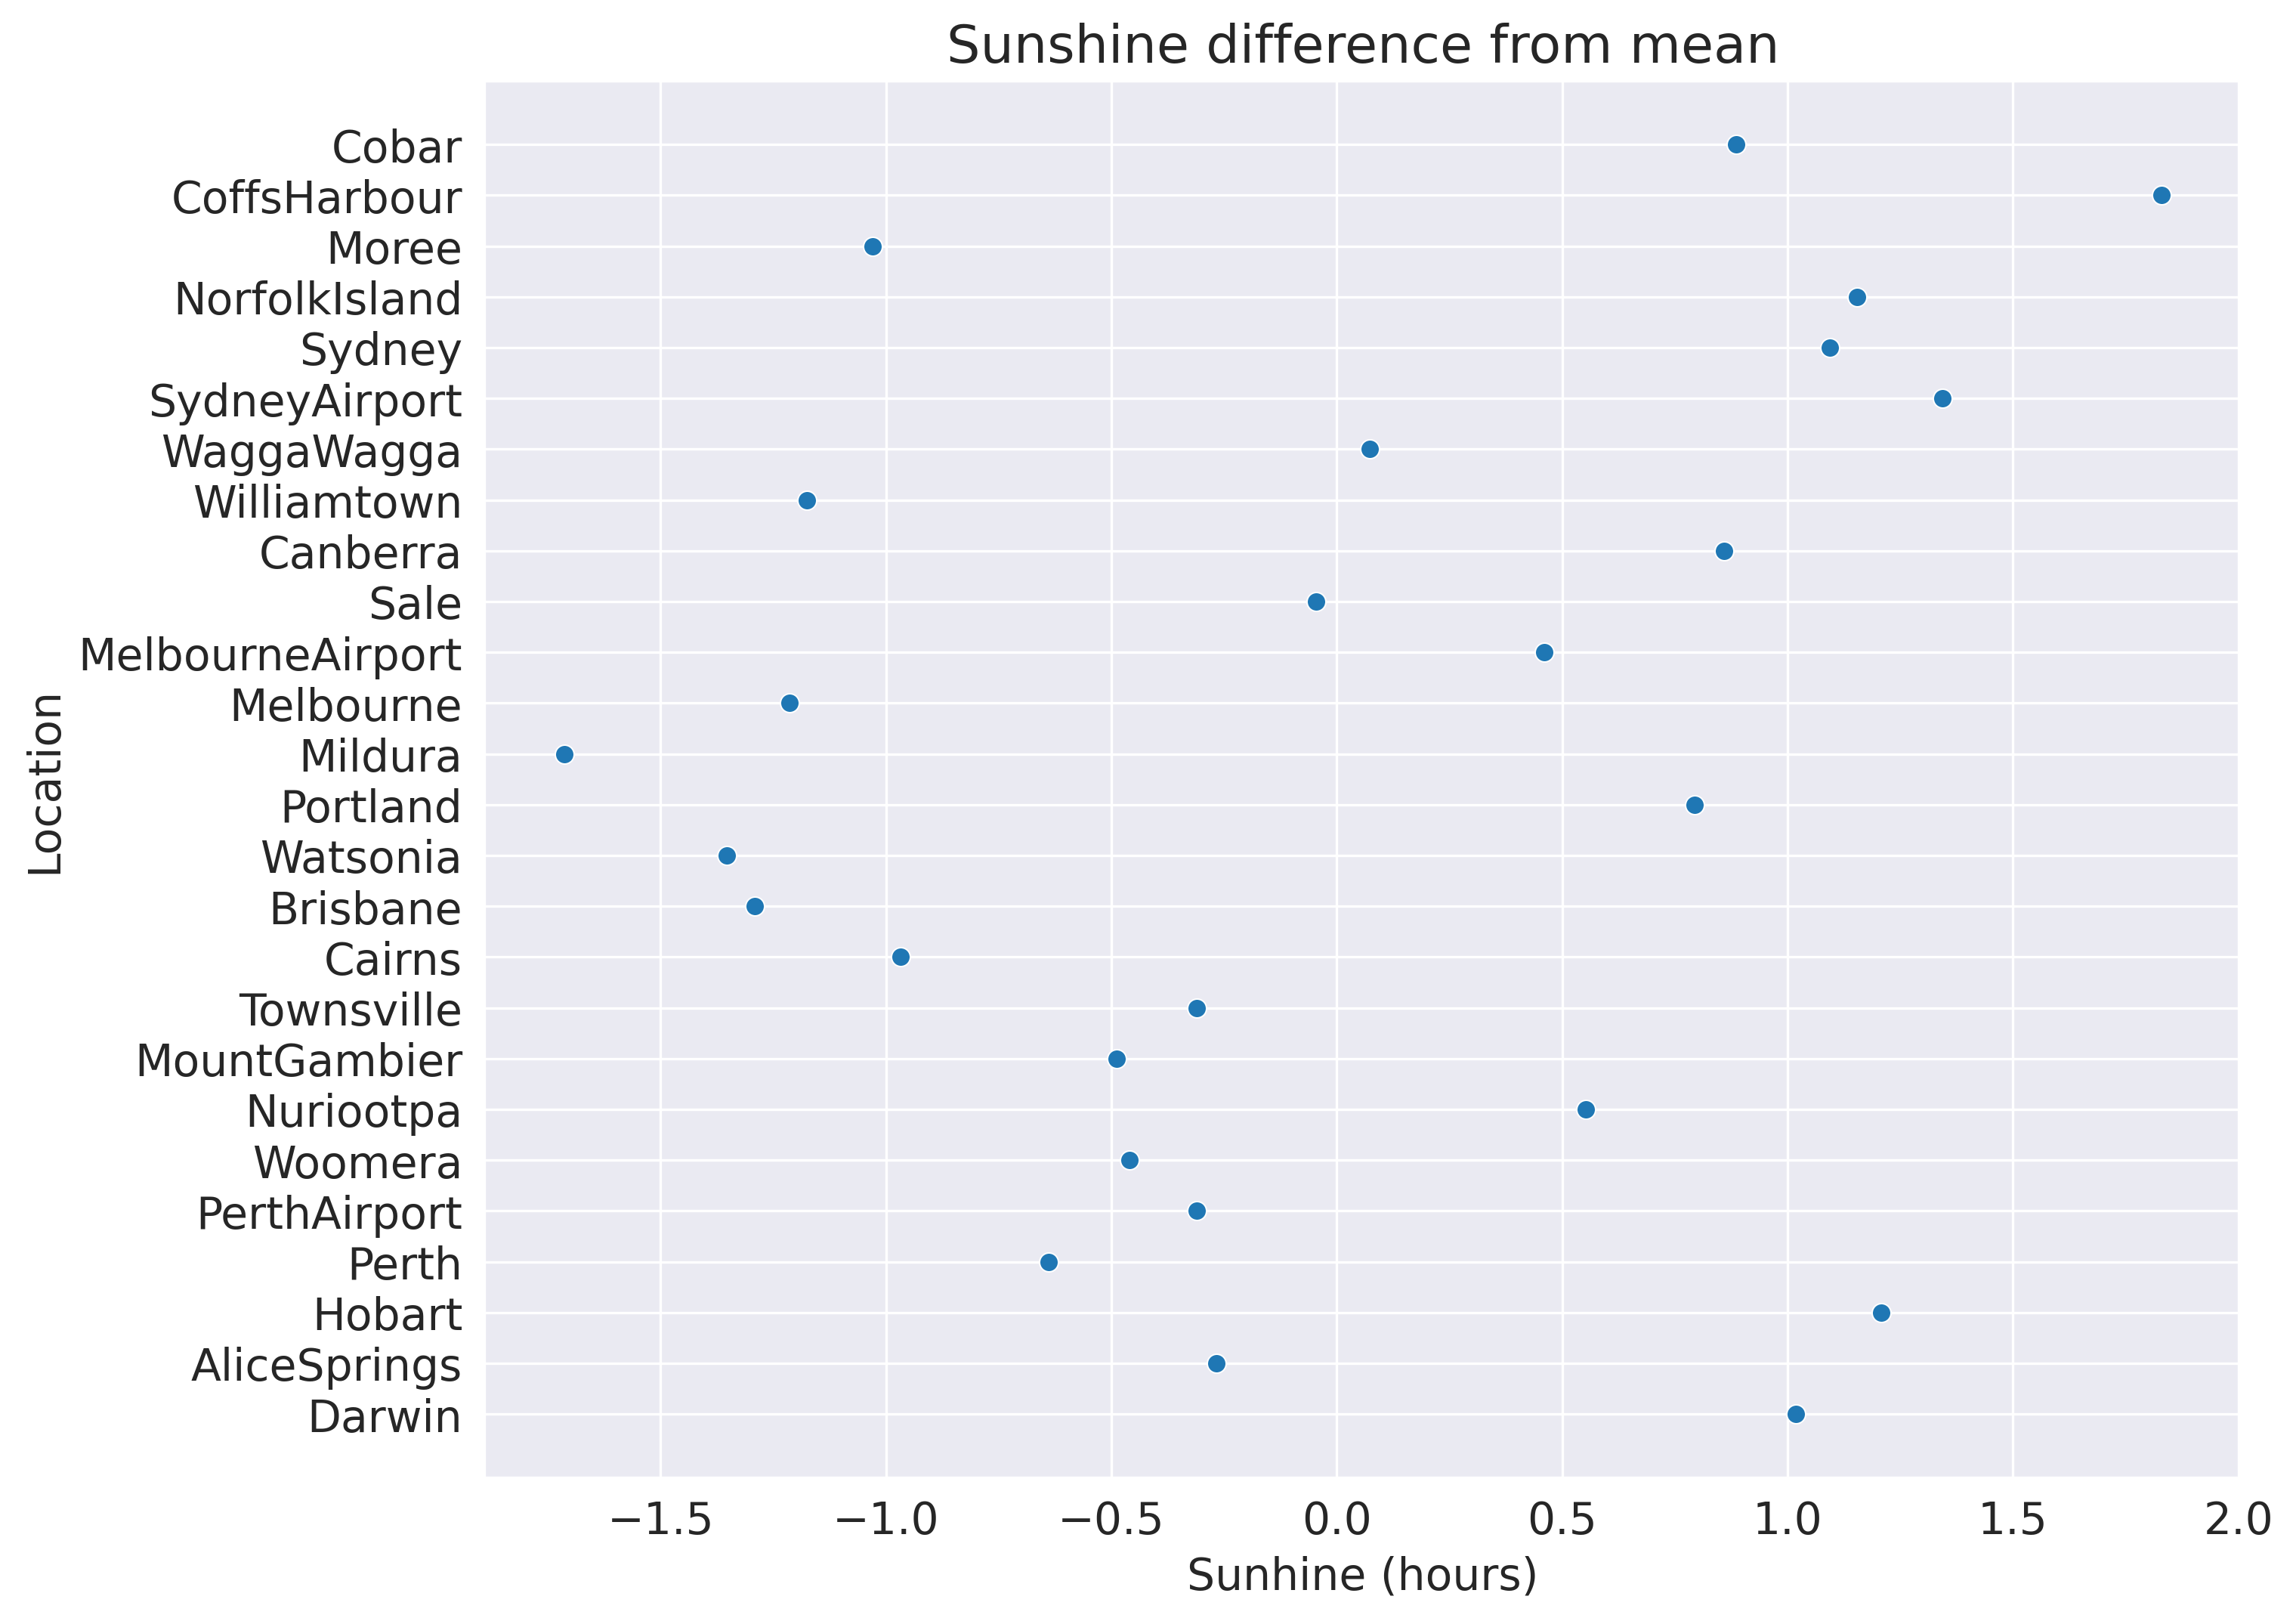
\includegraphics[width=.8\textwidth]{../figures/Sunshine.png}
        \caption{}
        \label{fig:sunshine}
    \end{subfigure}
    \begin{subfigure}{\textwidth}
        \centering
        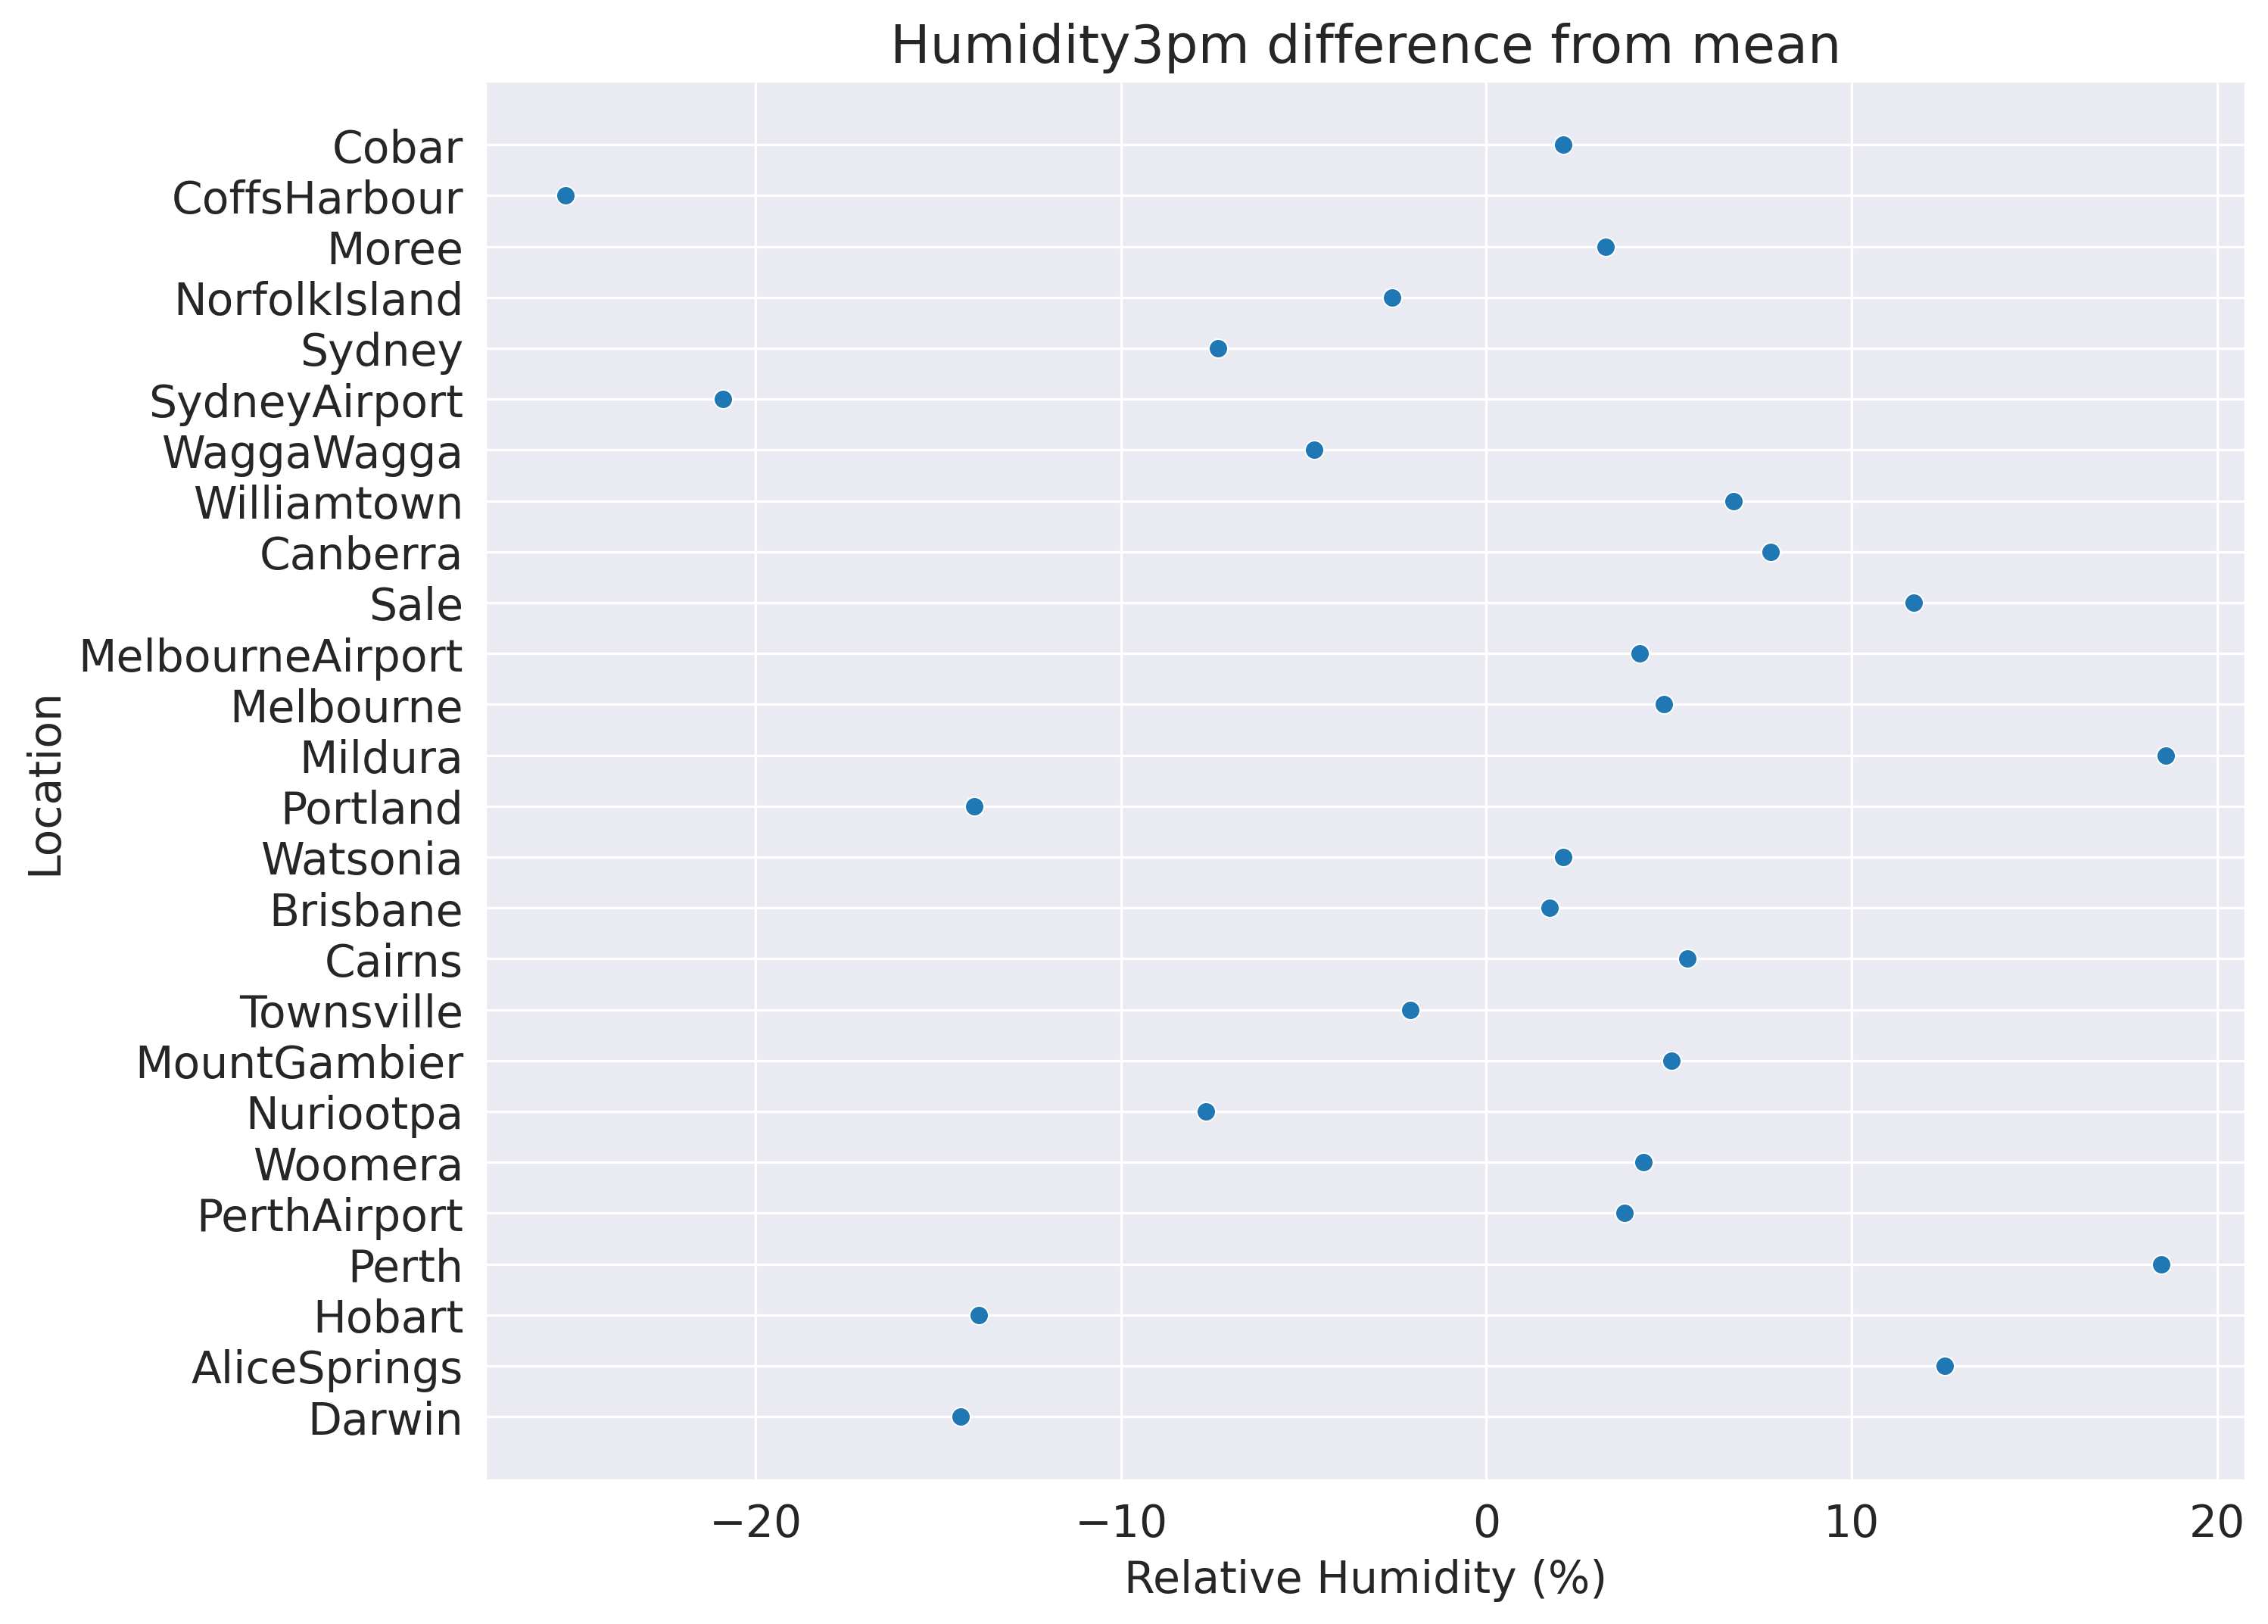
\includegraphics[width=.8\textwidth]{../figures/Relative_humidity3pm.png}
        \caption{}
        \label{fig:humidity}
    \end{subfigure}
    \caption{}
    \label{fig:features}
\end{figure}



Our first tests include a layer-neurons grid search for the Neural Network and a trees-depth grid search for the Random Forest. For the Neural Network and the logistic regression we perform the grid search using both ADAM and Stochastic Gradient Decent as optimizers for the gradient decent as seen in figure \ref{fig:cobar_grid}. Similarly, we see a Random Forest grid search in figure \ref{fig:cobar_grid_rf}.
\begin{figure}[H]
    \begin{subfigure}{.5\textwidth}
        \centering
        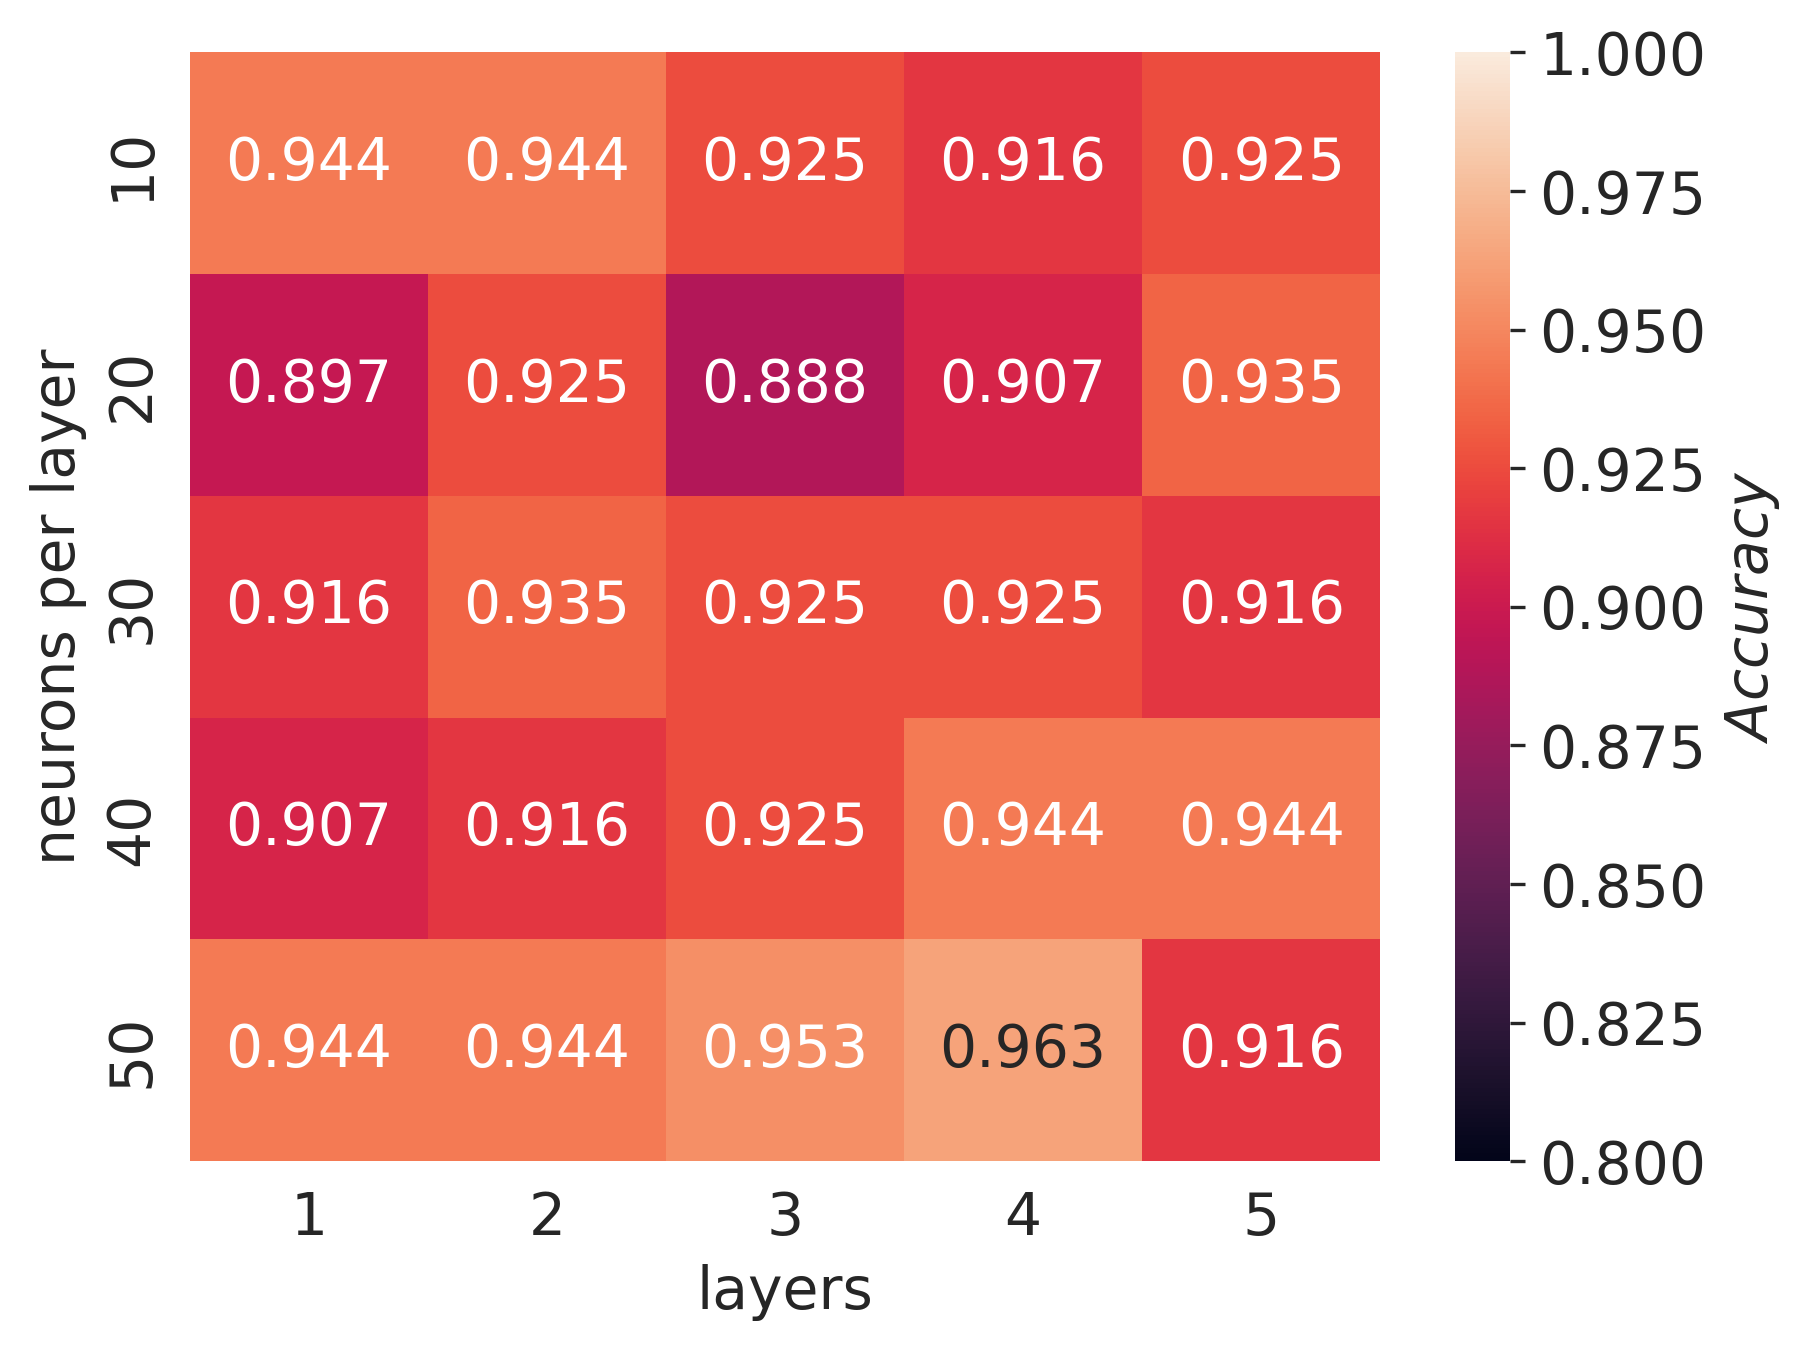
\includegraphics[width=\textwidth]{../figures/NN_grid_SGD_bootstrap_cobar.png}
        \caption{SGD}
        \label{fig:}
    \end{subfigure}
    \begin{subfigure}{.5\textwidth}
        \centering
        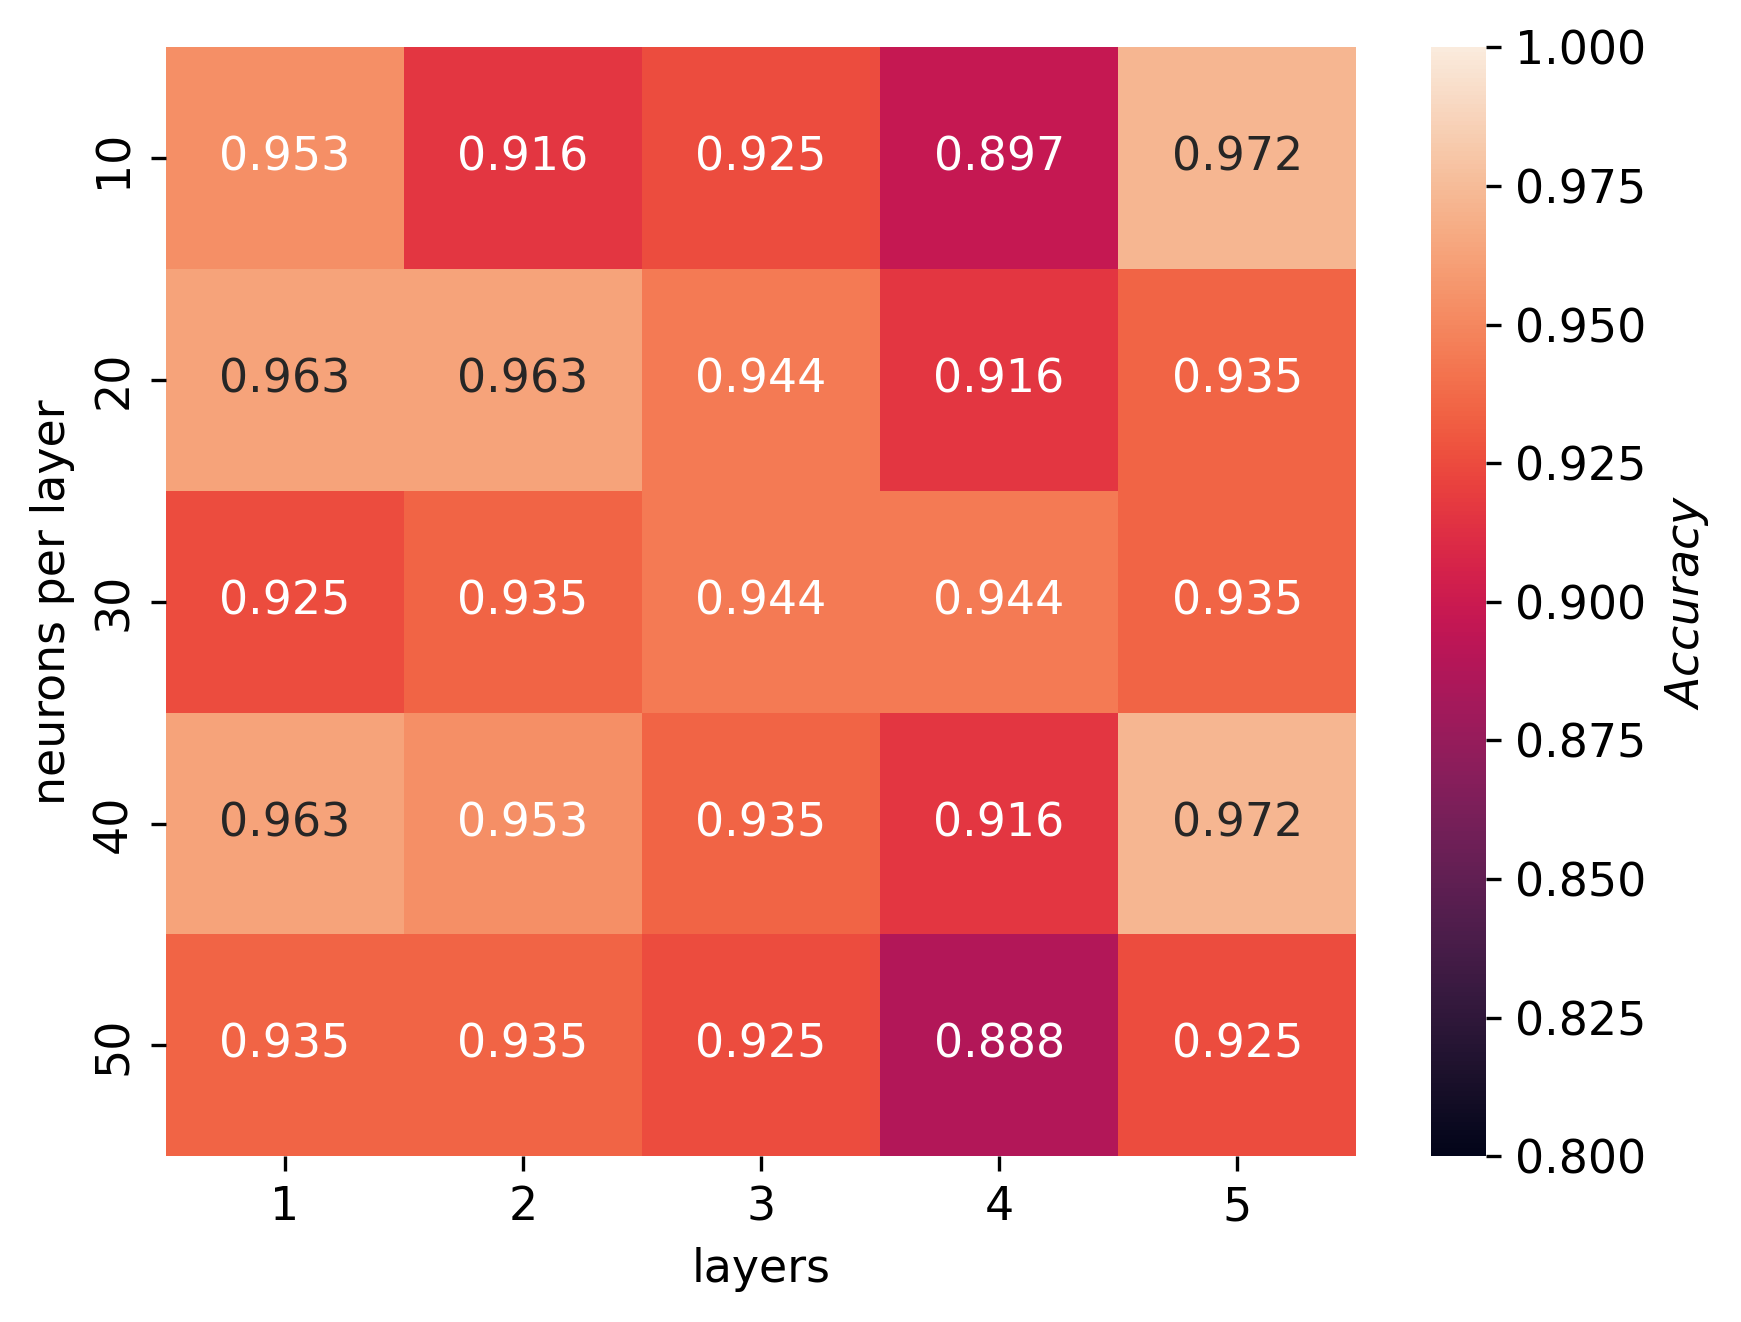
\includegraphics[width=\textwidth]{../figures/NN_grid_ADAM_bootstrap_cobar.png}
        \caption{ADAM}
        \label{fig:}
    \end{subfigure}
    \caption{Grid search for different learning rates ($\eta$) and L-2 norm ($\lambda$) for logistic regression. Momentum of 0.3, a batch size of 32 together with 100 epochs has been used.}
    \label{fig:cobar_grid}
\end{figure}
\begin{figure}[H]
    \begin{subfigure}{.5\textwidth}
        \centering
        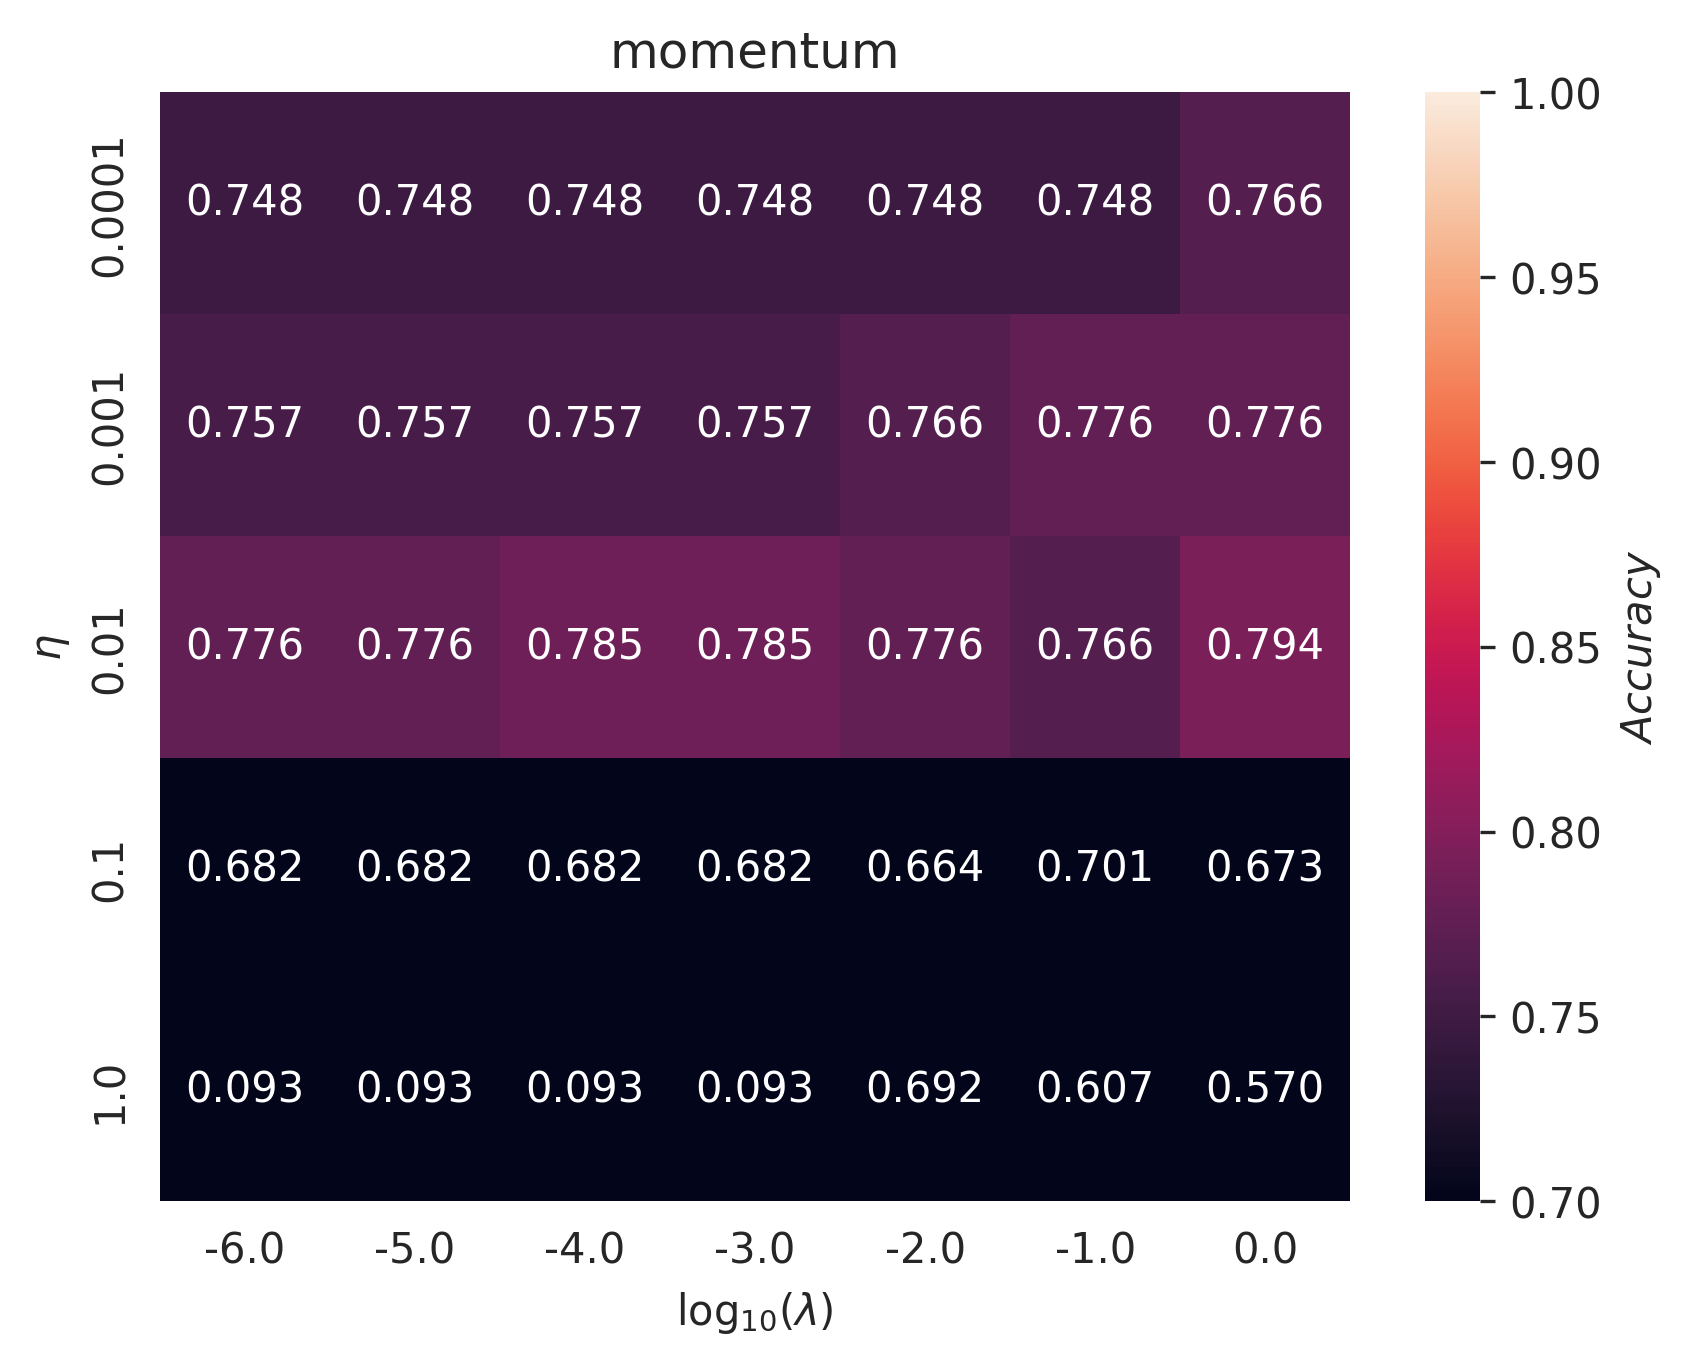
\includegraphics[width=\textwidth]{../figures/logreg_momentum_Cobar.png}
        \caption{SGD}
        \label{fig:}
    \end{subfigure}
    \begin{subfigure}{.5\textwidth}
        \centering
        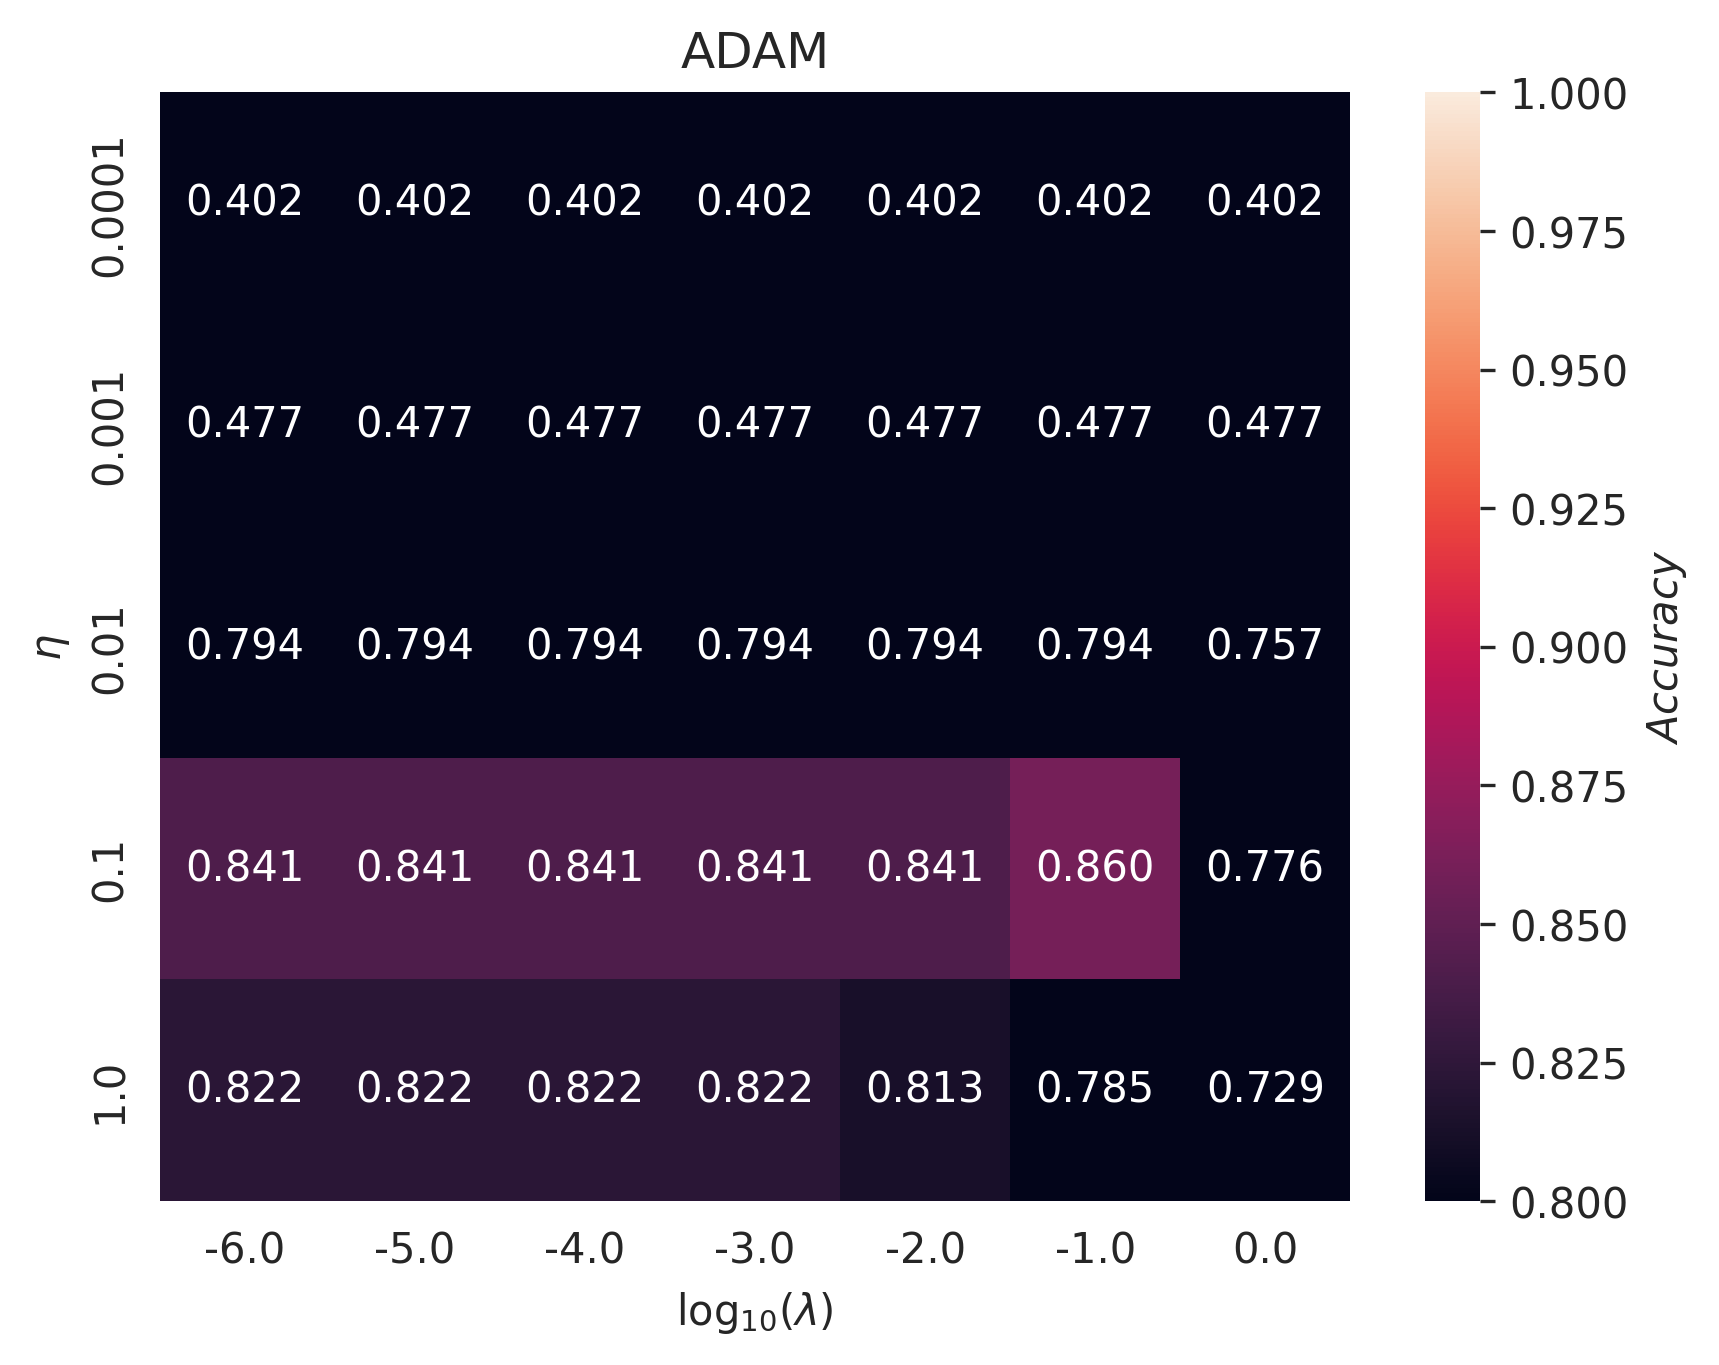
\includegraphics[width=\textwidth]{../figures/logreg_ADAM_Cobar.png}
        \caption{ADAM}
        \label{fig:}
    \end{subfigure}
    \caption{Grid search using 10 bootstrap iterations for different number of neurons and hidden layers in a tensorflow sequential Neural Network. ReLU has been used as activation for the hidden layers, and sigmoid for the output layer. Binary crossentropy has been used as loss function. A batch size of 32 together with 100 epochs has been used. All other parameters have been automatically chosen by tensorflow.}
    \label{fig:cobar_grid}
\end{figure}
\begin{figure}[H]
    \centering
    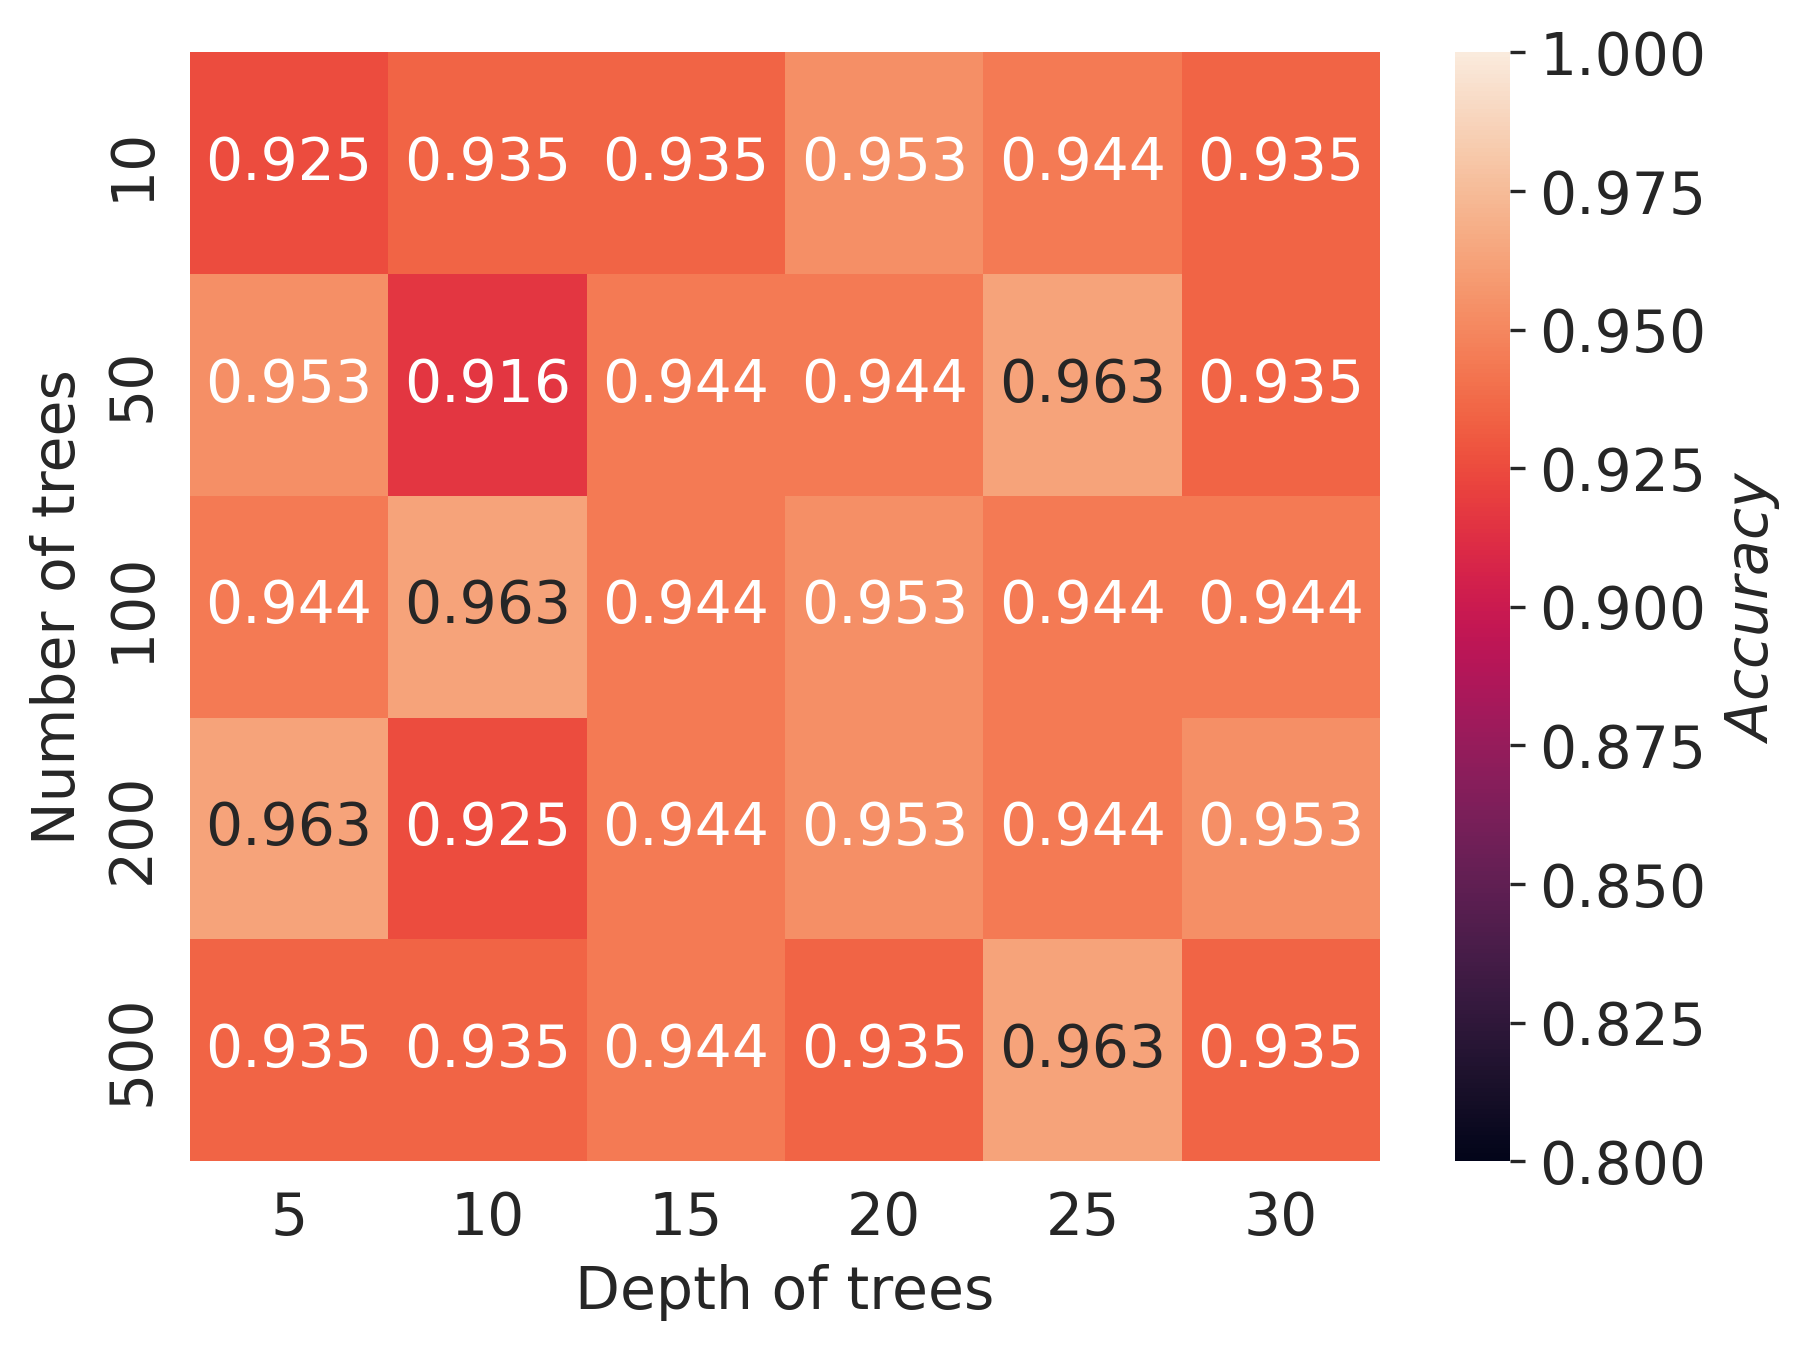
\includegraphics[width=0.5\textwidth]{../figures/RF_grid_bootstrap_cobar.png}
    \caption{Grid search using 10 bootstrap iterations for different number and depth of trees for a tensorflow Random Forest model. All other parameters are chosen automatically by tensorflow}
    \label{fig:cobar_grid_rf}
\end{figure}

We see that the performance in both figure \ref{fig:cobar_grid} and \ref{fig:cobar_grid_rf} vary depending on the parameters tested. The Neural Network performs slightly better than the Random Forest. The optimal parameters for the two models can be found below in table \ref{tab:grid_NN} and \ref{tab:grid_RF}.
\begin{table}[H]
    \caption{Optimal parameters found in grid search for Neural Network. 100 epochs and as batch size of 32 has been used. Other parameters are automatically chosen by tensorflow}
    \label{tab:grid_NN}
    \centering
    \begin{tabular}{|l|l|l|l|l|}
        \hline
        \textbf{Train Data}      & \textbf{Test Data}         & \textbf{Neurons} & \textbf{Layers} & \textbf{Accuracy} \\
        \hline
        80\% split of Cobar data & 20\% split of Cobar data   & 20               & 2               & 97.2\%            \\
        \hline
        100\% of Cobar data      & 100\% of CoffsHarbour data & 20               & 2               & 74.5\%            \\
        \hline
        100\% of Cobar data      & 100\% of Darwin data       & 20               & 2               & 75.5\%            \\
        \hline
        80\% split of all data   & 20\% split of all data     & 50               & 4               & 85.7\%            \\
        \hline
        80\% of full data        & 20\% of Cobar data         & 50               & 4               & 92.5\%            \\
        \hline
        80\% of full data        & 20\% of Darwin data        & 50               & 4               & 85.3\%            \\
        \hline
    \end{tabular}
\end{table}

\subsection{Full data analysis} % (fold)
\label{sub:Full data analysis}
We look at a dataset containing all weather stations and perform a grid search for the random forest as shown in figure \ref{fig:grid_full}.
\begin{figure}[H]
    \begin{subfigure}{.5\textwidth}
        \centering
        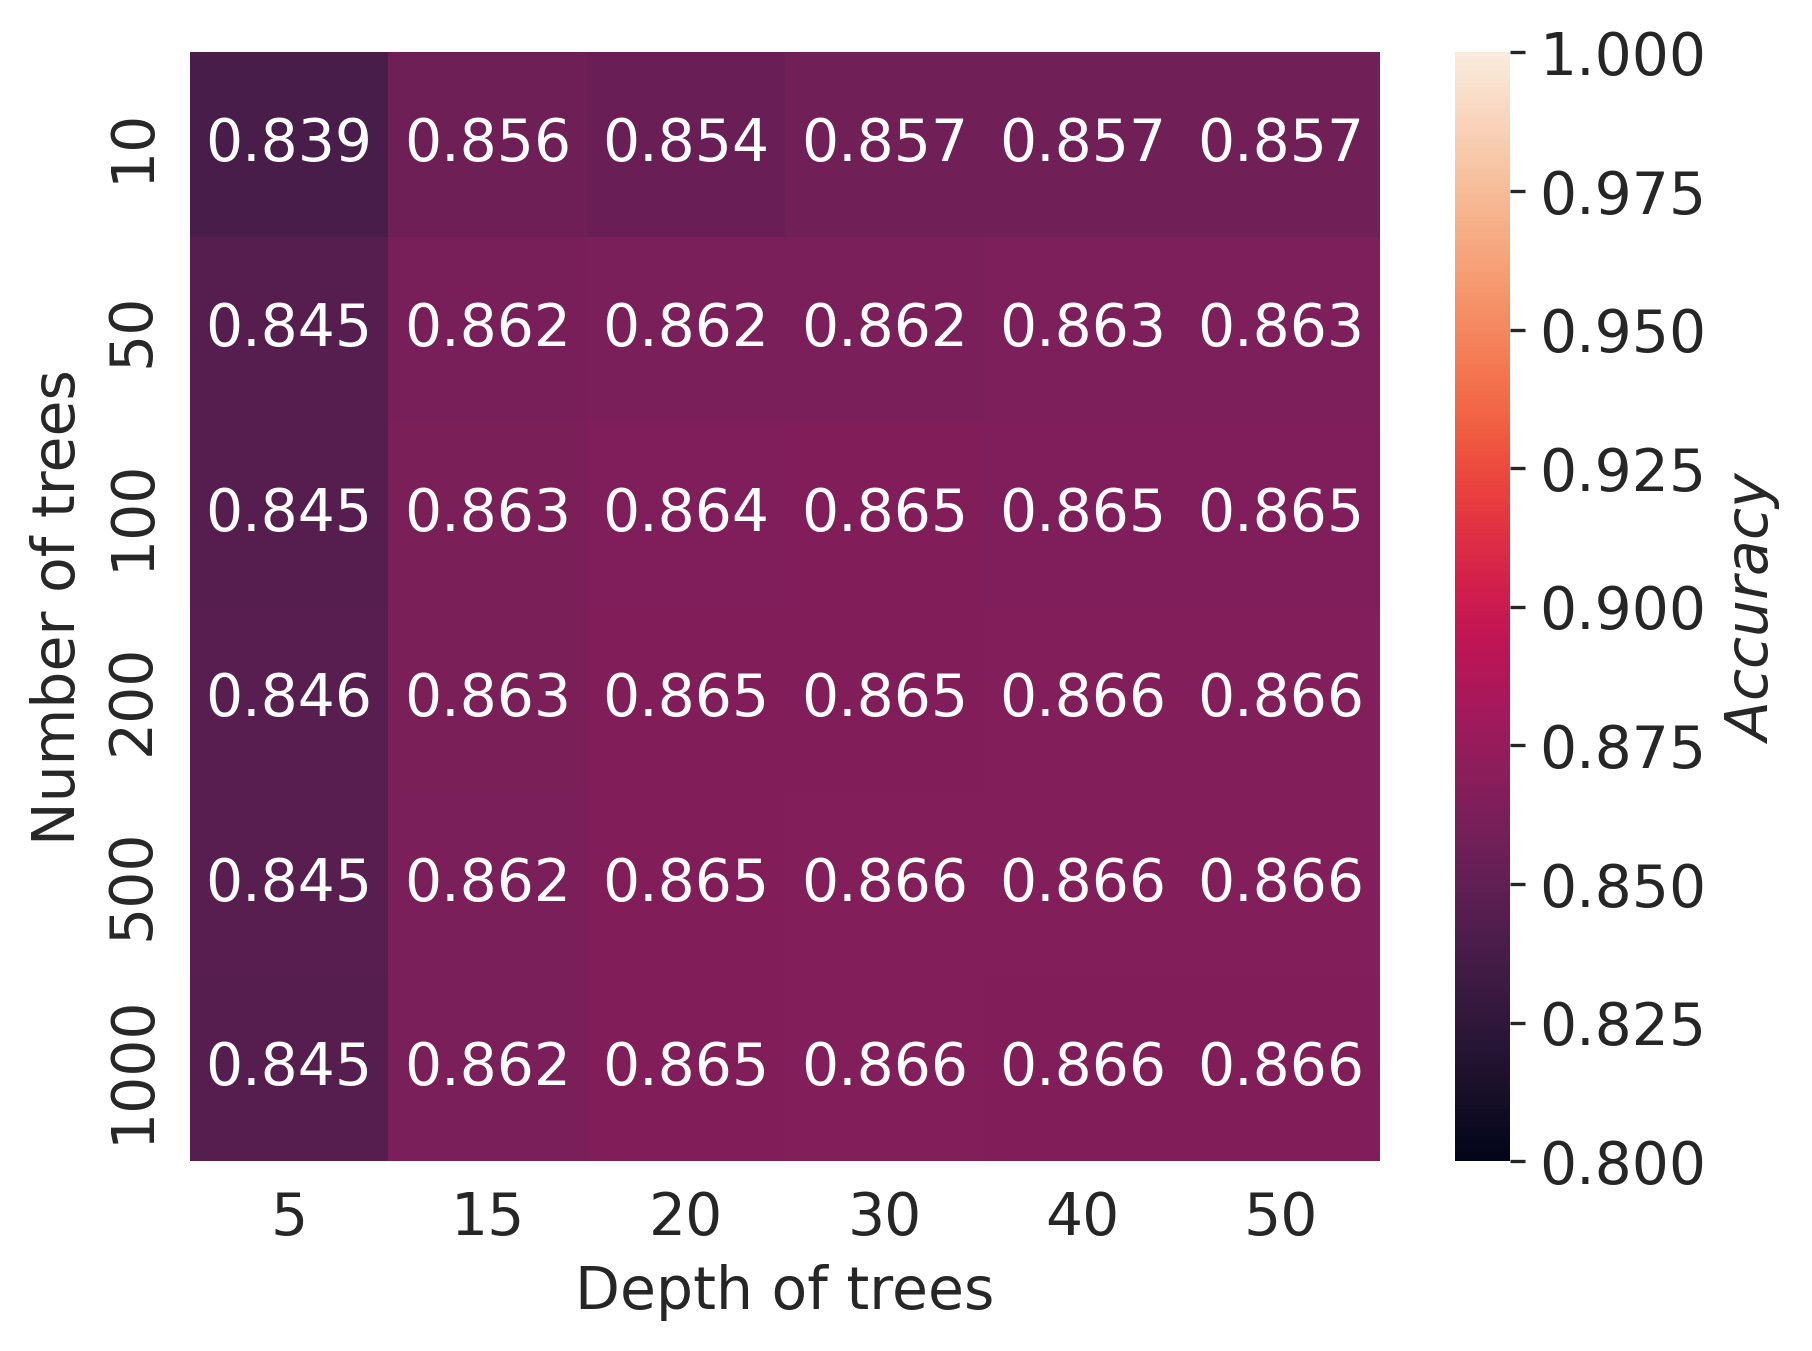
\includegraphics[width=\textwidth]{../figures/RF_grid_all.png}
        \caption{Random Forest}
        \label{fig:rf_full}
    \end{subfigure}
    \begin{subfigure}{.5\textwidth}
        \centering
        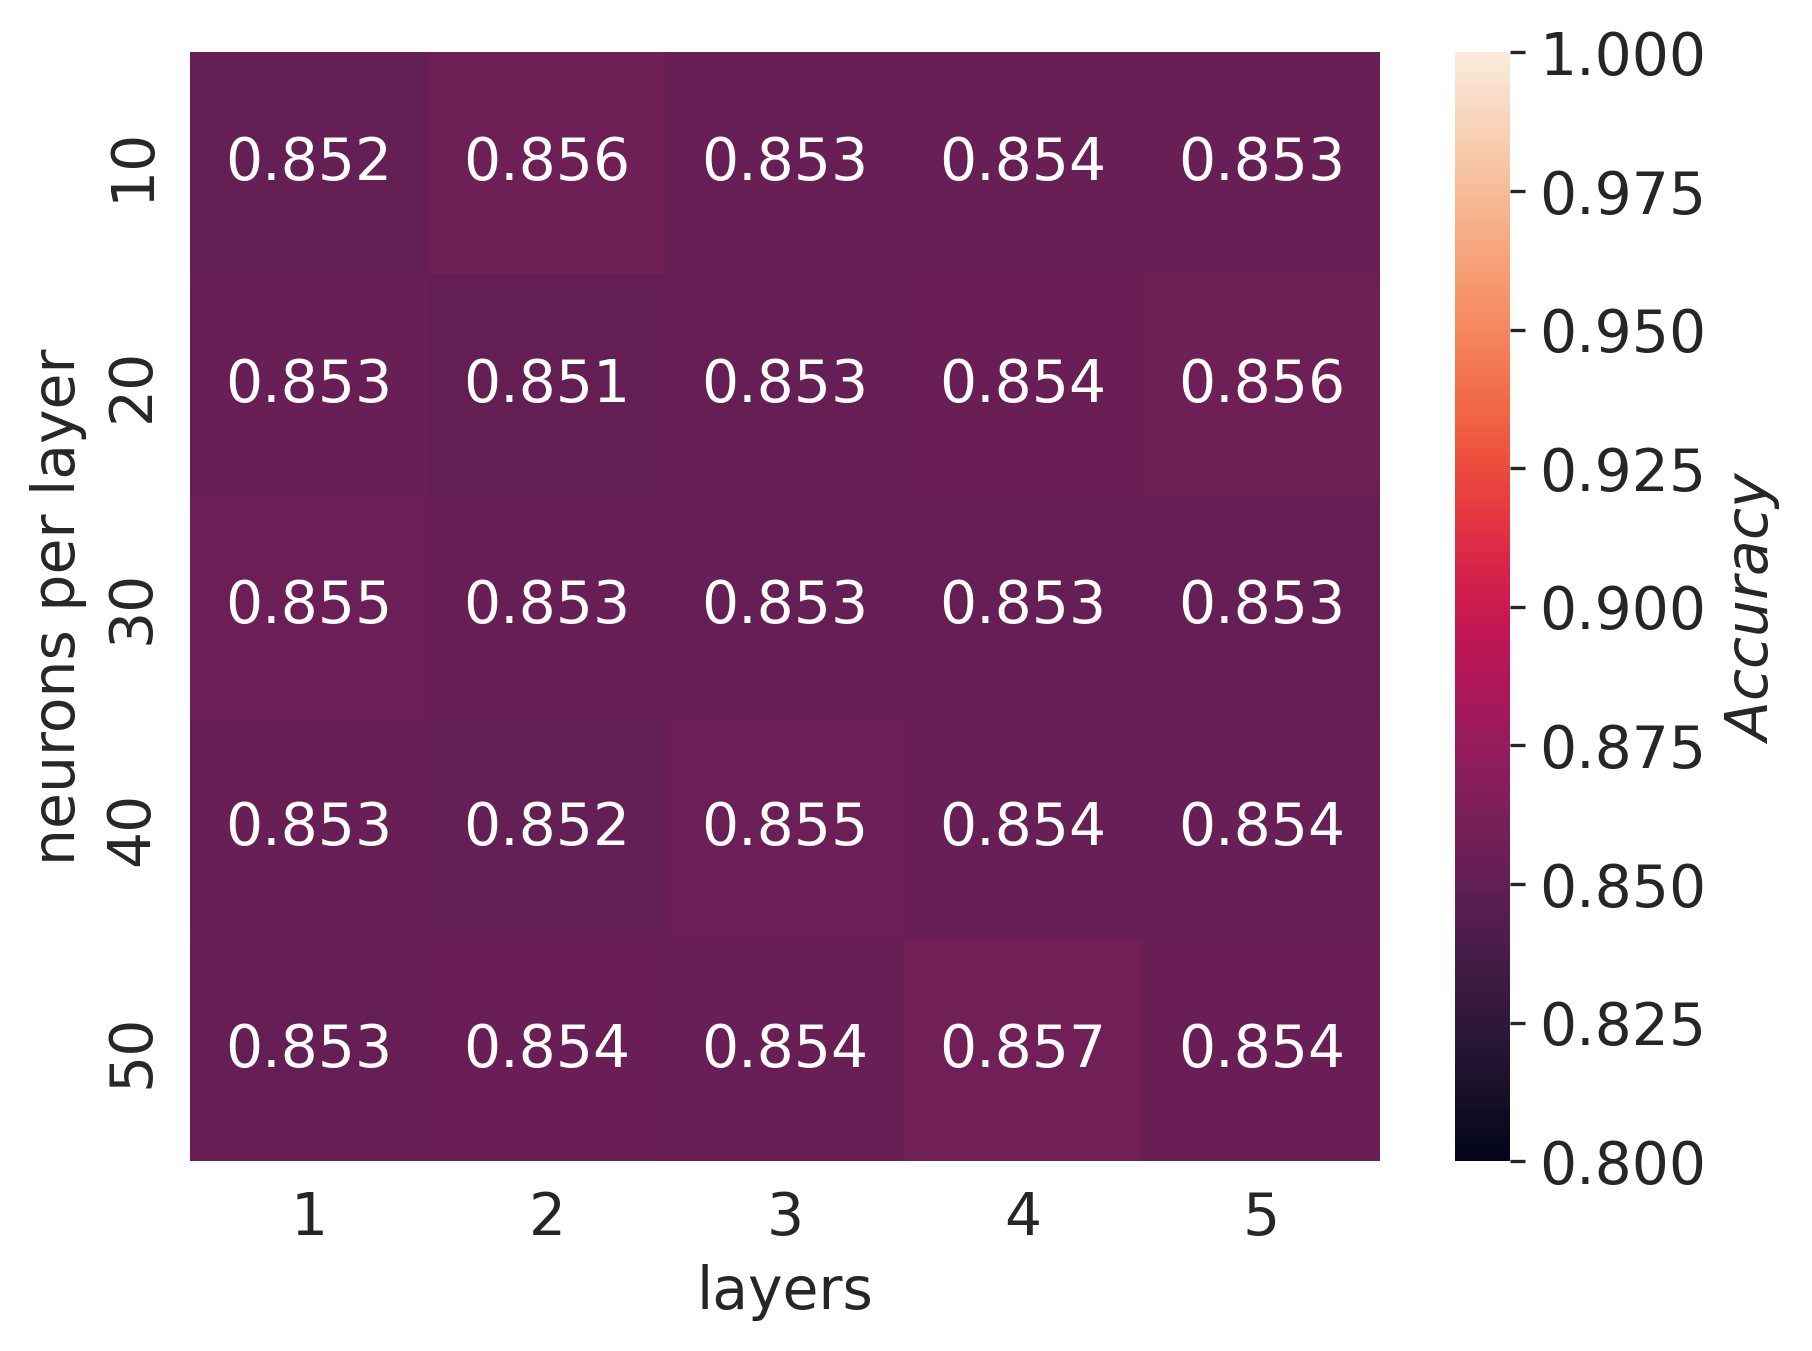
\includegraphics[width=\textwidth]{../figures/NN_grid_ADAM_bootstrap_all.png}
        \caption{Neural Network with ADAM}
        \label{fig:NN_full}
    \end{subfigure}
    \caption{Grid search using 10 bootstrap iterations for a Neural Network and a Random Forest. For the Neural Network has ReLU been used as activation for the hidden layers, and sigmoid for the output layer. Binary crossentropy has been used as loss function. A batch size of 320 together with 100 epochs has been used. All other parameters for both the Neural Network and the Random Forest have been automatically chosen by tensorflow.}
    \label{fig:grid_full}
\end{figure}

We see in \ref{fig:rf_full} that more trees and a larger depth generally equals a more accurate model. For the Neural Network wee see more variation and not a clear tendency with more neurons and layers equalling a more accurate model. The parameters used, and the highest accuracy is shown in table \ref{tab:grid_RF}.

\begin{table}[H]
    \caption{Optimal parameters found in grid search for Random Forest. Other parameters are chosen automatically by tensorflow.}
    \label{tab:grid_RF}
    \centering
    \begin{tabular}{|l|l|l|l|l|}
        \hline
        \textbf{Train Data}      & \textbf{Test Data}         & \textbf{Trees} & \textbf{Depth} & \textbf{Accuracy} \\
        \hline
        80\% split of Cobar data & 20\% split of Cobar data   & 100            & 10             & 96.3\%            \\
        \hline
        80\% split of all data   & 20\% split of all data     & 500            & 20             & 86.6\%            \\
        \hline
        100\% of Cobar data      & 100\% of CoffsHarbour data & 100            & 10             & 77.9\%            \\
        \hline
        100\% of Cobar data      & 100\% of Darwin data       & 100            & 10             & 82.4\%            \\
        \hline
        80\% of full data        & 20\% of Cobar data         & 500            & 20             & 94.4\%            \\
        \hline
        80\% of full data        & 20\% of Darwin data        & 500            & 20             & 87.4\%            \\
        \hline
    \end{tabular}
\end{table}
% subsection Full data analysis (end)
\begin{itemize}
    \item initializing a pandas dataframe,
    \item remove all rows with at least one measurement missing,
    \item Look at sized of data from the different stations - spanning from 534 to 3062 for 22 features
    \item will need package tensorflowdecisionforests
    \item Bootstrap to reduce overfitting and improve generalization ability
    \item perform bootstrap on different weight and bias initializations
    \item Current small scale weather stations - lots of data
    \item Compairison between areas - assume that masked values not happen at specific times and weather conditions
    \item Relative high accuracy on Cobar test data - Climate maybe largest factor not weather station.  - train model on data on the other side of the world - help weather predictions here?
\end{itemize}


\newpage
\appendix
\section{Dataset}
\label{app:dataset}
\begin{table}[H]
    \begin{small}
        \caption{Description of dataset features to predict the last feature "RainTomorrow" if it is going to rain tomorrow or not }
        \label{tab:features}
        \begin{center}
            \begin{tabular}{|l|l|l|}
                \hline
                \textbf{Feature} & \textbf{desctiption}                                 & \textbf{Unit}           \\
                \hline
                \hline
                Location         & Common name of the weather station                   & name                    \\
                \hline
                MinTemp          & Minimum temperature                                  & degrees Celcius         \\
                \hline
                MaxTemp          & Maximum temperature                                  & degrees Celcius         \\
                \hline
                Rainfall         & Amount of rainfall recorded in the day               & mm                      \\
                \hline
                Evaporation      & The "Class A" pan evaporation in the 24 hours        & mm                      \\
                \hline
                Sunshine         & Number of hours with bright sunshine in the day      & hours                   \\
                \hline
                WindGustDir      & direction of the strongest wind gust in the 24 hours & 16-wind compass rose    \\
                \hline
                WindGustSpeed    & Speed of the strongest wind gust in the 24 hours     & km/h                    \\
                \hline
                WindDir9am       & wind direction at 9am                                & 16-wind compass rose    \\
                \hline
                WindDir3pm       & wind direction at 3pm                                & 16-wind compass rose    \\
                \hline
                WindSpeed9am     & Wind speed at 9am                                    & km/h                    \\
                \hline
                WindSpeed3pm     & Wind speed at 3pm                                    & km/h                    \\
                \hline
                Humidity9am      & Relative humidity at 9am                             & percent                 \\
                \hline
                Humidity3pm      & Relative humidity at 3pm                             & percent                 \\
                \hline
                Pressure9am      & Pressure reduced to mean sea level at 9am            & hPa                     \\
                \hline
                Pressure3pm      & Pressure reduced to mean sea level at 3pm            & hPa                     \\
                \hline
                Cloud9am         & Fraction of sky covered by clouds at 9am             & oktas (units of eights) \\
                \hline
                Cloud3pm         & Fraction of sky covered by clouds at 3pm             & oktas (units of eights) \\
                \hline
                Temp9am          & Temperature at 9am                                   & degrees Celcius         \\
                \hline
                Temp3pm          & Temperature at 3pm                                   & degrees Celcius         \\
                \hline
                RainToday        & Rain exceeding 1mm over 24 hours today               & Yes or No               \\
                \hline
                RainTomorrow     & Rain exceeding 1mm over 24 hours tomorrow            & Yes or No               \\
                \hline
            \end{tabular}
        \end{center}
    \end{small}
\end{table}

\end{document}